% !TeX program = xelatex
\documentclass[aspectratio=169,10pt]{beamer}

\usepackage{fontspec}
\setsansfont{Noto Sans}
\setmainfont{Noto Sans}
\usepackage{booktabs}
\usepackage{tabularx}
\usepackage{array}
\usepackage{tikz}
\usetikzlibrary{arrows.meta,positioning,shapes.geometric}
\usepackage{graphicx}
\usepackage{ragged2e}

\definecolor{uetblue}{HTML}{0C4F7E}
\definecolor{deepblue}{HTML}{123B5A}
\definecolor{lightblue}{HTML}{E8F3FA}
\definecolor{cyan}{HTML}{00A6D6}
\definecolor{green}{HTML}{159C68}
\definecolor{amber}{HTML}{D88900}
\definecolor{red}{HTML}{C9485B}
\definecolor{ink}{HTML}{17324A}
\definecolor{muted}{HTML}{566B7D}
\definecolor{linegray}{HTML}{CAD7E0}

\setbeamercolor{normal text}{fg=ink,bg=white}
\setbeamercolor{structure}{fg=uetblue}
\setbeamercolor{frametitle}{fg=deepblue,bg=white}
\setbeamercolor{itemize item}{fg=cyan}
\setbeamercolor{itemize subitem}{fg=cyan}
\setbeamertemplate{navigation symbols}{}
\setbeamertemplate{itemize item}{\raise0.15ex\hbox{\scriptsize$\blacktriangleright$}}
\setbeamertemplate{itemize subitem}{\raise0.1ex\hbox{\tiny$\bullet$}}
\setbeamertemplate{frametitle}{%
  \vspace{0.16cm}\hspace{0.16cm}\insertframetitle\par
  \vspace{-0.08cm}\hspace{0.16cm}\color{uetblue}\rule{0.965\paperwidth}{0.7pt}}
\setbeamertemplate{footline}{%
  \leavevmode\hbox{%
    \begin{beamercolorbox}[wd=.84\paperwidth,ht=2.6ex,dp=1.2ex,leftskip=.45cm]{normal text}%
      \fontsize{6.3}{7.2}\selectfont\color{muted}\insertshorttitle
    \end{beamercolorbox}%
    \begin{beamercolorbox}[wd=.13\paperwidth,ht=2.6ex,dp=1.2ex,rightskip=.35cm plus1fil]{normal text}%
      \fontsize{7}{8}\selectfont\color{muted}\insertframenumber/\inserttotalframenumber
    \end{beamercolorbox}}}
\setbeamersize{text margin left=0.50cm,text margin right=0.50cm}

\newcommand{\good}[1]{\textcolor{green}{\textbf{#1}}}
\newcommand{\warn}[1]{\textcolor{amber}{\textbf{#1}}}
\newcommand{\risk}[1]{\textcolor{red}{\textbf{#1}}}
\newcommand{\keynum}[1]{\textcolor{uetblue}{\textbf{#1}}}
\newcommand{\source}[1]{\vfill{\fontsize{5.7}{6.5}\selectfont\color{muted}Nguồn: #1}}
\newcommand{\smallbullet}{\setlength{\itemsep}{0.15em}\setlength{\parskip}{0pt}}

\newenvironment{bluebox}[1]{%
  \begin{beamercolorbox}[rounded=true,shadow=true,sep=0.18cm]{block body}%
  {\color{uetblue}\textbf{#1}}\par\vspace{0.08cm}\color{ink}%
}{\end{beamercolorbox}}

\setbeamercolor{block body}{fg=ink,bg=lightblue}
\setbeamercolor{block title}{fg=white,bg=uetblue}

\title[Ba đóng góp và bằng chứng thực nghiệm]{Hệ thống phát hiện Ransomware dựa trên Phân tích đa tầng,\\
tích hợp Học tích cực và Kiểm chứng độ trung thực XAI}
\author{Học viên: Lưu Văn Doanh}
\institute{GVHD: PGS.TS. Trương Ninh Thuận\\Trường Đại học Công nghệ -- ĐHQGHN}
\date{Hà Nội, 2026}

\begin{document}

% 1
\begin{frame}[plain]
  \begin{tikzpicture}[remember picture,overlay]
    \fill[uetblue] (current page.north west) rectangle ([yshift=-0.11cm]current page.north east);
    \node[anchor=north west] at ([xshift=0.55cm,yshift=-0.35cm]current page.north west)
      {
\includegraphics[width=0.72cm]{assets/uet_logo.png}};
    \node[anchor=north east] at ([xshift=-0.55cm,yshift=-0.35cm]current page.north east)
      {
\includegraphics[width=0.72cm]{assets/vnu_logo.png}};
  \end{tikzpicture}
  \centering
  \vspace{0.55cm}
  {\small\bfseries ĐẠI HỌC QUỐC GIA HÀ NỘI\\TRƯỜNG ĐẠI HỌC CÔNG NGHỆ}\par
  \vspace{0.35cm}
  {\fontsize{21}{24}\selectfont\bfseries\color{uetblue} BÁO CÁO LUẬN VĂN THẠC SĨ}\par
  \vspace{0.28cm}
  {\fontsize{9.2}{11}\selectfont Ngành: Kỹ thuật phần mềm \hspace{1.0cm} Mã số: 8480103.01}\par
  \vspace{0.38cm}
  {\fontsize{14.7}{18}\selectfont\bfseries\color{deepblue}\inserttitle}\par
  \vspace{0.42cm}
  {\small\insertauthor\par\insertinstitute}\par
  \vfill
  {\scriptsize\color{muted}Ba đóng góp và bằng chứng thực nghiệm có thể truy nguyên}\par
  \vspace{0.12cm}
  {\scriptsize\insertdate}
\end{frame}

% 2
\begin{frame}[t]{Mạch trình bày}
\begin{columns}[T,onlytextwidth]
\column{0.48\textwidth}
\begin{bluebox}{Bốn nội dung chính}
\begin{enumerate}\smallbullet
  \item Bài toán và khoảng trống nghiên cứu.
  \item Kiến trúc và \textbf{ba đóng góp giữ nguyên}.
  \item Bằng chứng thực nghiệm cho từng đóng góp.
  \item Ý nghĩa, giới hạn và mức đóng góp tổng thể.
\end{enumerate}
\end{bluebox}

\column{0.48\textwidth}
\begin{bluebox}{Nguyên tắc trình bày}
\begin{itemize}\smallbullet
  \item Không dùng Accuracy đơn lẻ để chứng minh hiệu quả.
  \item Mỗi số liệu truy về một artifact đã kiểm tra.
  \item Báo cả kết quả thuận lợi và kết quả chưa hỗ trợ giả thuyết.
  \item Nêu đúng quy mô của từng thực nghiệm và khoảng tin cậy.
\end{itemize}
\end{bluebox}
\end{columns}

\vspace{0.50cm}
\centering
\begin{tikzpicture}[node distance=0.55cm]
\foreach \x/\t/\c in {0/Bài toán/uetblue,3.0/Kiến trúc/cyan,6.0/Bằng chứng/green,9.0/Kết luận/amber}{
  \node[draw=\c,rounded corners=2pt,minimum width=2.25cm,minimum height=0.62cm,text=ink,font=\small\bfseries] (n\x) at (\x,0) {\t};}
\draw[-{Stealth[length=2mm]},line width=0.7pt,color=muted] (1.15,0)--(1.85,0);
\draw[-{Stealth[length=2mm]},line width=0.7pt,color=muted] (4.15,0)--(4.85,0);
\draw[-{Stealth[length=2mm]},line width=0.7pt,color=muted] (7.15,0)--(7.85,0);
\end{tikzpicture}
\end{frame}

% 3
\begin{frame}[t,shrink=6]{Bài toán và động lực nghiên cứu}
\begin{columns}[T,onlytextwidth]
\column{0.57\textwidth}
\textbf{Bài toán vận hành}
\begin{itemize}\smallbullet
  \item Phân tích tĩnh nhanh, nhưng dễ suy giảm trước packing, obfuscation và API nạp động.
  \item Phân tích động quan sát được hành vi, nhưng tốn thời gian và tài nguyên.
  \item Hệ thống cần cập nhật trước mẫu mới mà không gán nhãn toàn bộ dữ liệu.
  \item Lời giải thích SHAP cần được kiểm tra bằng hành vi mô hình, thay vì chỉ trực quan hóa.
\end{itemize}

\vspace{0.25cm}
\begin{bluebox}{Câu hỏi nghiên cứu trung tâm}
Làm thế nào kết hợp tín hiệu tĩnh--động, lựa chọn nhãn hiệu quả và kiểm chứng lời giải thích trong cùng một quy trình có thể đánh giá?
\end{bluebox}

\column{0.39\textwidth}
\begin{tikzpicture}[node distance=0.36cm]
\node[draw=uetblue,fill=lightblue,rounded corners,minimum width=4.15cm,minimum height=0.85cm,align=center] (a) {\textbf{Hiệu năng phát hiện}\\AUC, AP, FPR/TPR};
\node[draw=green,fill=green!8,rounded corners,minimum width=4.15cm,minimum height=0.85cm,align=center,below=of a] (b) {\textbf{Chi phí vận hành}\\phân tích động, nhãn, overhead};
\node[draw=amber,fill=amber!8,rounded corners,minimum width=4.15cm,minimum height=0.85cm,align=center,below=of b] (c) {\textbf{Độ tin cậy giải thích}\\deletion và stability};
\end{tikzpicture}
\end{columns}
\end{frame}

% 4
\begin{frame}[t]{Khoảng trống nghiên cứu và điểm khác biệt}
\scriptsize
\renewcommand{\arraystretch}{1.32}
\begin{tabularx}{\textwidth}{>{\bfseries}p{2.3cm} X X}
\toprule
Hướng hiện có & Giới hạn thường gặp & Phần luận văn bổ sung \\
\midrule
Dung hợp tĩnh--động & Trọng số cố định; khó phản ứng khi độ tin cậy thay đổi & \textbf{PID Fusion}: trọng số thay đổi theo bất đồng và trạng thái chuỗi \\
Active Learning & Chủ yếu dựa trên uncertainty xác suất & \textbf{XAI-Guided AL}: thêm Directional Entropy $H$ và SHAP Variance $V$ \\
SHAP cho mã độc & Thường dừng ở heatmap hoặc danh sách đặc trưng & \textbf{Fidelity Framework}: deletion control và độ ổn định thứ hạng \\
Đánh giá hệ thống & Nhấn mạnh một metric tổng hợp & Báo riêng ranking, low-FPR, chi phí nhãn và overhead \\
\bottomrule
\end{tabularx}

\vspace{0.42cm}
\begin{bluebox}{Phạm vi khoa học}
Hệ thống hướng tới ransomware; bằng chứng hiện tại được đo trên dữ liệu mã độc Windows có nguồn và định danh. Không suy rộng sang ransomware/zero-day nếu nhãn nguồn chưa hỗ trợ.
\end{bluebox}
\end{frame}

% 5
\begin{frame}[t]{Kiến trúc hệ thống đa tầng}
\centering
\begin{tikzpicture}[
  box/.style={draw=uetblue,fill=lightblue,rounded corners=2pt,minimum width=2.00cm,minimum height=0.72cm,align=center,font=\scriptsize},
  support/.style={draw=green,fill=green!8,rounded corners=2pt,minimum width=3.00cm,minimum height=0.70cm,align=center,font=\scriptsize},
  arr/.style={-{Stealth[length=2mm]},thick,color=muted},node distance=0.42cm]
\node[box] (pe) {Tệp PE};
\node[box,right=of pe] (static) {LightGBM\\$p_s$ + TreeSHAP};
\node[box,right=of static] (gate) {Cổng bất định};
\node[box,right=of gate] (dyn) {Chuỗi API\\$p_d$};
\node[box,right=of dyn,draw=cyan,line width=1.1pt] (pid) {\textbf{PID Fusion}\\$p_s+p_d$};
\node[box,right=of pid] (out) {Quyết định\\+ giải thích};
\draw[arr] (pe)--(static); \draw[arr] (static)--(gate); \draw[arr] (gate)--(dyn);
\draw[arr] (dyn)--(pid); \draw[arr] (pid)--(out);
\draw[arr,bend right=34] (static.south) to node[below,font=\tiny]{ngoài vùng bất định} (out.south);
\node[support,below=1.18cm of static] (al) {\textbf{XAI-Guided AL}\\chọn mẫu $\rightarrow$ gán nhãn $\rightarrow$ học lại};
\node[support,below=1.18cm of pid,draw=amber] (fid) {\textbf{Fidelity/Consistency}\\kiểm tra lời giải thích};
\draw[arr,color=green] (static.south)--(al.north);
\draw[arr,color=green] (al.east)--++(0.45,0)|-(static.south east);
\draw[arr,color=amber] (out.south)--(fid.north);
\end{tikzpicture}

\vspace{0.48cm}
\begin{columns}[T,onlytextwidth]
\column{0.32\textwidth}\centering
\textcolor{cyan}{\textbf{PID}}\\[-1mm]\scriptsize Điều chỉnh luật dung hợp
\column{0.32\textwidth}\centering
\textcolor{green}{\textbf{Active Learning}}\\[-1mm]\scriptsize Tối ưu ngân sách nhãn
\column{0.32\textwidth}\centering
\textcolor{amber}{\textbf{Fidelity}}\\[-1mm]\scriptsize Kiểm tra chất lượng giải thích
\end{columns}
\end{frame}

% 6
\begin{frame}[t,shrink=7]{Đóng góp 1 — Luật dung hợp PID theo chuỗi sự kiện}
\begin{columns}[T,onlytextwidth]
\column{0.54\textwidth}
\begin{bluebox}{Cập nhật trọng số động}
\[
e_t=p_d(t)-p_s,\qquad
u_t=K_p e_t+K_i\sum_{\tau\le t}e_\tau+K_d(e_t-e_{t-1})
\]
\[
w_{t+1}=\operatorname{clip}(w_t+u_t),\qquad
p_f(t)=w_t p_s+(1-w_t)p_d(t)
\]
\small
Trục thời gian là \textbf{số lời gọi API đã quan sát}: $t\in\{5,10,15,20\}$, không phải số giây.
\end{bluebox}

\column{0.42\textwidth}
\small
\begin{bluebox}{Vì sao cần ba thành phần?}
\begin{itemize}\smallbullet
  \item $P$: phản ứng với bất đồng hiện tại.
  \item $I$: tích lũy bất đồng có hệ thống.
  \item $D$: phản ứng với tốc độ thay đổi tín hiệu.
\end{itemize}
\end{bluebox}

\vspace{0.15cm}
\begin{bluebox}{Cách chứng minh}
Không suy luận hiệu quả từ công thức. So sánh Static, Dynamic, Average, Fixed, P, PI và PID trên cùng outer folds; dùng bootstrap ghép cặp cho chênh lệch.
\end{bluebox}
\end{columns}
\end{frame}

% 6
\begin{frame}[t,shrink=5]{Ba đóng góp của luận văn}
\begin{columns}[T,onlytextwidth]
\column{0.32\textwidth}
\begin{bluebox}{1. PID Fusion}
\small
\begin{itemize}\smallbullet
  \item Dung hợp $p_s$ và $p_d$ theo tiến trình.
  \item Ablation: Static, Dynamic, Fixed, P, PI, PID.
  \item Đo AUC/AP, FPR/TPR và độ nhạy.
\end{itemize}
\good{Đã đo: cohort ghép cặp $n=199$.}
\end{bluebox}

\column{0.32\textwidth}
\begin{bluebox}{2. XAI-Guided AL}
\small
\begin{itemize}\smallbullet
  \item $S=0{,}3\hat U+0{,}4\hat H+0{,}3\hat V$.
  \item So Random, U, U+H, U+V, XAI-full.
  \item Đo AULC, budget-to-target và overhead.
\end{itemize}
\good{Trạng thái: đã xác nhận.}
\end{bluebox}

\column{0.32\textwidth}
\begin{bluebox}{3. Fidelity Framework}
\small
\begin{itemize}\smallbullet
  \item Che top-$|$SHAP$|$ và random cùng $k$.
  \item Mean/median baseline; $k=10,25,50$.
  \item Đo deletion và rank stability.
\end{itemize}
\good{Trạng thái: đã xác nhận.}
\end{bluebox}
\end{columns}

\vspace{0.40cm}
\centering\small
\textbf{Không tổng hợp OFS} khi chưa có chuẩn hóa và trọng số chung được kiểm định; báo riêng từng thành phần để tránh điểm số tùy ý.
\end{frame}

% 7
\begin{frame}[t,shrink=6]{Thiết lập thực nghiệm có thể truy nguyên}
\begin{columns}[T,onlytextwidth]
\column{0.49\textwidth}
\begin{bluebox}{AL và Fidelity — thực nghiệm xác nhận}
\small
\begin{itemize}\smallbullet
  \item \textbf{2.000} dòng EMBER 2018; \textbf{2.381} đặc trưng.
  \item SHA-256 và feature hash đã đối chiếu theo từng dòng.
  \item 5 outer folds; 5 seed trong mỗi fold: \textbf{25} cặp fold--seed.
  \item Test không tham gia chọn mẫu, threshold hoặc tham số.
\end{itemize}
\end{bluebox}

\column{0.49\textwidth}
\begin{bluebox}{PID — thực nghiệm ghép cặp tĩnh--động}
\small
\begin{itemize}\smallbullet
  \item MalBehavD-V1: \textbf{199/200} mẫu usable (100 benign, 99 malware).
  \item Kênh động: chuỗi API ở mốc 5, 10, 15, 20 sự kiện.
  \item Kênh tĩnh: 199 đặc trưng cấu trúc PE an toàn.
  \item 5 outer folds; bootstrap ghép cặp 1.000 lần.
\end{itemize}
\end{bluebox}
\end{columns}

\vspace{0.33cm}
\begin{bluebox}{Quy tắc đánh giá}
Khóa split trước khi đo; chọn gain/trọng số/ngưỡng trên train--validation; lưu dự đoán từng mẫu, cấu hình, manifest và SHA-256 artifact; báo giới hạn dữ liệu cùng kết quả.
\end{bluebox}
\source{results/confirmatory\_20261019\_ember\_identity; results/measured\_20261020\_malbehavd\_pid\_pilot200.}
\end{frame}

% 8
\begin{frame}[t,shrink=8]{Đóng góp 1 — PID Fusion: kết quả trên 199 mẫu}
\begin{columns}[T,onlytextwidth]
\column{0.61\textwidth}
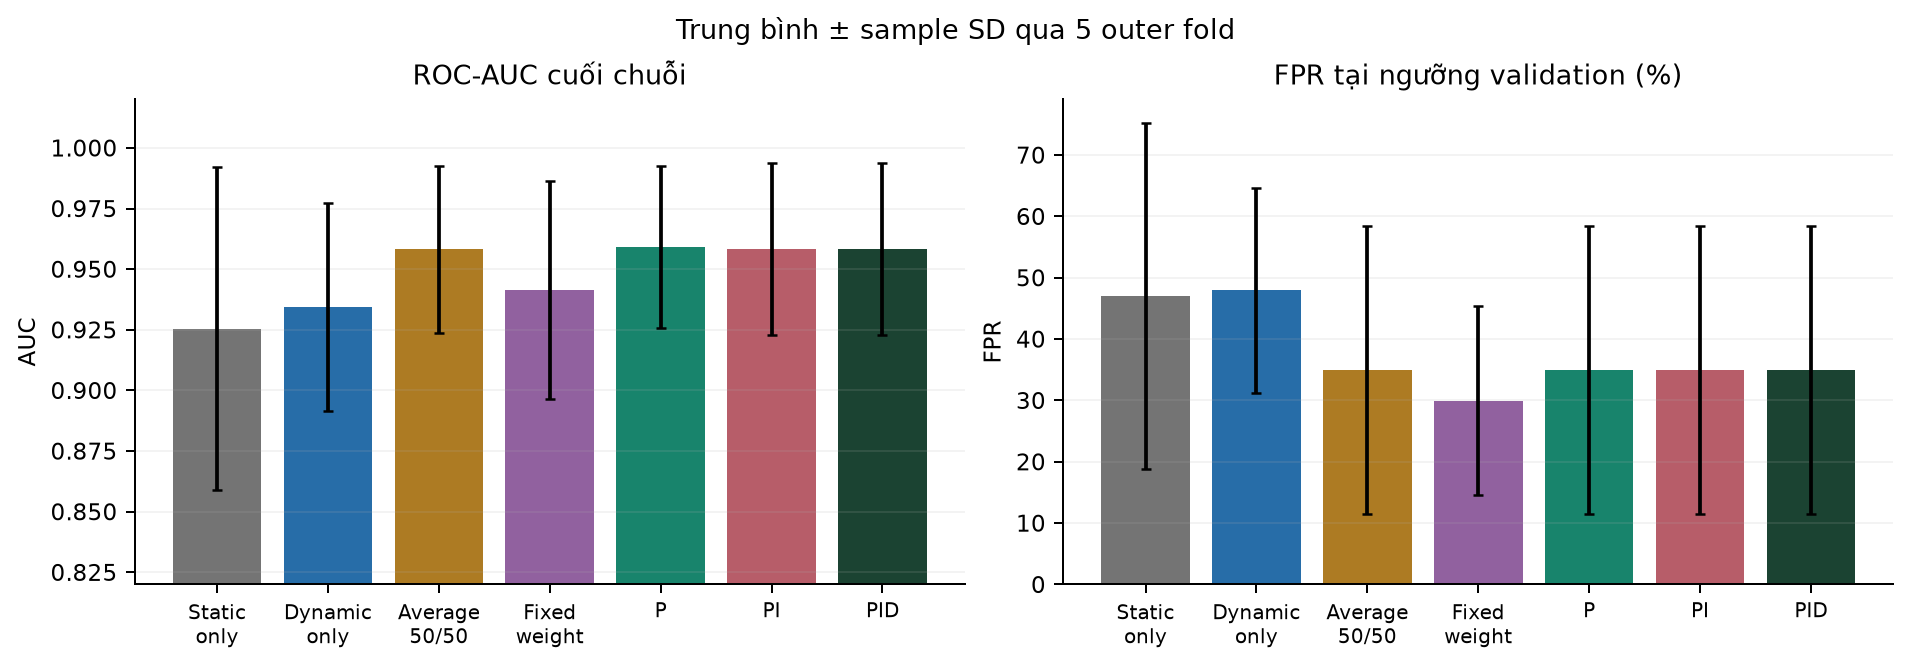
\includegraphics[width=\linewidth]{assets/pid_metrics.png}

\column{0.37\textwidth}
\small
\begin{bluebox}{Kết quả chính}
\begin{itemize}\smallbullet
  \item Static: \keynum{0,9254} AUC.
  \item Dynamic: \keynum{0,9345} AUC.
  \item P: \keynum{0,9592}; PI/PID: \keynum{0,9583}.
  \item PID -- Fixed: $\Delta$AUC \keynum{+0,0130}; CI 95\% $[-0,0086; +0,0409]$.
  \item $\Delta$TPR \good{+4,10 pp}; $\Delta$FPR \risk{+5,06 pp}.
\end{itemize}
\end{bluebox}

\vspace{0.15cm}
\begin{bluebox}{Diễn giải}
Dung hợp thích nghi cải thiện ranking trên cohort này. PI và PID không đổi quyết định nào; dữ liệu hiện tại chưa chứng minh lợi ích riêng của thành phần D hoặc khả năng giảm FPR.
\end{bluebox}
\end{columns}
\source{event\_pid\_table.tex; paired\_bootstrap\_pid\_minus\_fixed.json; $n=199$, 5 outer folds.}
\end{frame}

% 10
\begin{frame}[t,shrink=8]{PID Ablation — Thành phần nào tạo ra khác biệt?}
\begin{columns}[T,onlytextwidth]
\column{0.60\textwidth}
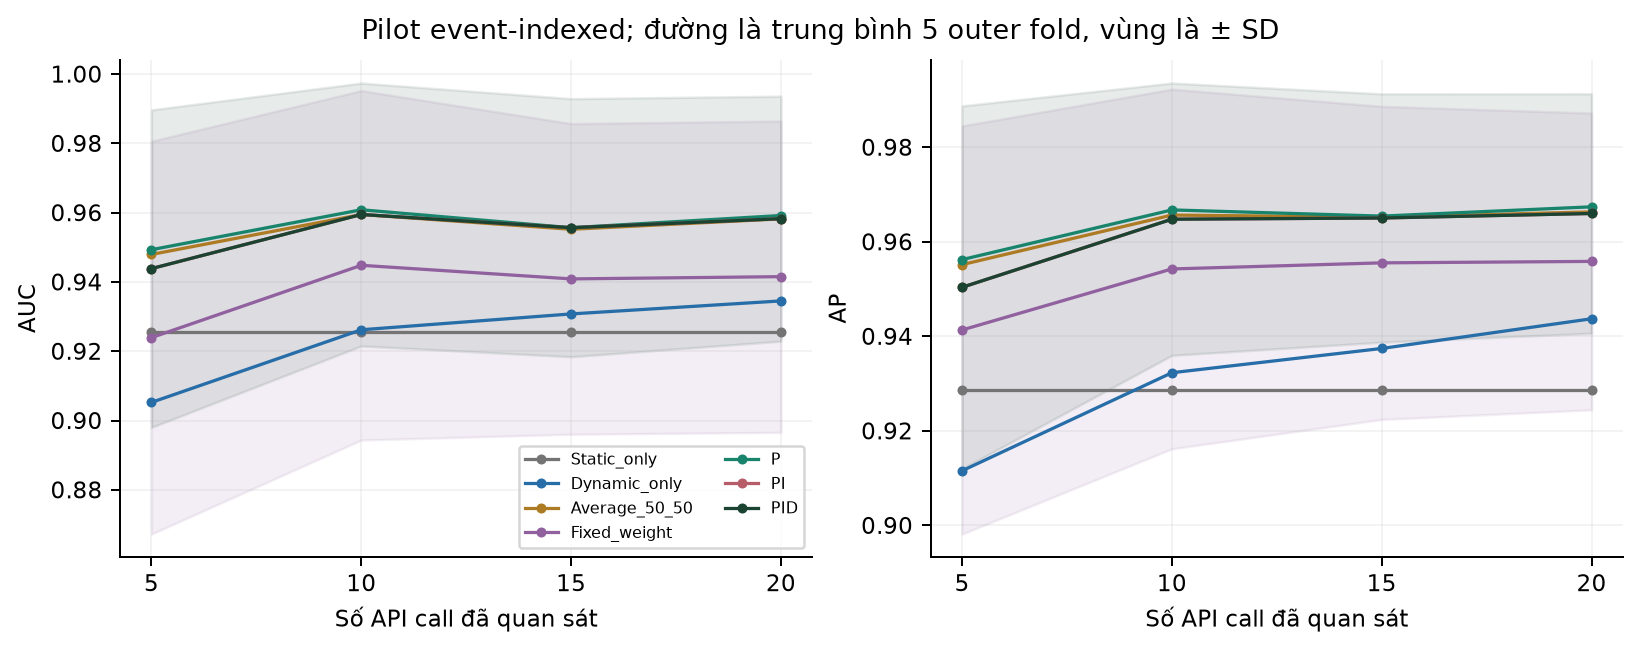
\includegraphics[width=\linewidth,height=0.67\textheight,keepaspectratio]{assets/event_pid_trajectory.png}

\column{0.38\textwidth}
\small
\begin{bluebox}{So sánh AUC}
\begin{itemize}\smallbullet
  \item Static: \keynum{0,9254}.
  \item Dynamic: \keynum{0,9345}.
  \item Average: \keynum{0,9582}.
  \item Fixed: \keynum{0,9415}.
  \item P: \good{0,9592}.
  \item PI/PID: \keynum{0,9583}.
\end{itemize}
\end{bluebox}

\vspace{0.12cm}
\begin{bluebox}{Kết luận ablation}
Lợi ích chính đến từ \textbf{dung hợp hai nguồn} và phản ứng $P$. Với bốn mốc sự kiện, $I$ và $D$ chưa tạo khác biệt đo được; vì vậy không gán công lao giảm FPR cho PID đầy đủ.
\end{bluebox}
\end{columns}
\end{frame}

% 9
\begin{frame}[t,shrink=7]{Đóng góp 2 — Từ XAI đến quyết định gán nhãn}
\begin{columns}[T,onlytextwidth]
\column{0.54\textwidth}
\begin{bluebox}{Điểm truy vấn}
\[
S(x)=0{,}3\widehat U(x)+0{,}4\widehat H(x)+0{,}3\widehat V(x)
\]
\small
\begin{itemize}\smallbullet
  \item $U$: bất định xác suất dự đoán.
  \item $H$: entropy hướng của đóng góp SHAP, đo xung đột giữa nhóm đặc trưng.
  \item $V$: độ phân tán độ lớn SHAP.
\end{itemize}
\end{bluebox}

\column{0.42\textwidth}
\begin{bluebox}{Thiết kế so sánh công bằng}
\small
\begin{itemize}\smallbullet
  \item Cùng initial set, pool, batch và ngân sách.
  \item So Random, Uncertainty, U+H, U+V và XAI-full.
  \item Human-in-the-loop: chiến lược chỉ \textbf{chọn mẫu}; không tự sinh nhãn.
  \item Đo AULC, số nhãn tới mục tiêu và query overhead.
\end{itemize}
\end{bluebox}
\end{columns}

\vspace{0.20cm}
\begin{bluebox}{Giả thuyết kiểm chứng}
Nếu tín hiệu giải thích hữu ích, chiến lược có $H/V$ phải đạt cùng mức hiệu năng với ít nhãn hơn hoặc cải thiện toàn bộ đường học, thay vì chỉ tăng AUC ở vòng cuối.
\end{bluebox}
\end{frame}

% 10
\begin{frame}[t,shrink=8]{Đóng góp 2 — XAI-Guided Active Learning}
\begin{columns}[T,onlytextwidth]
\column{0.64\textwidth}
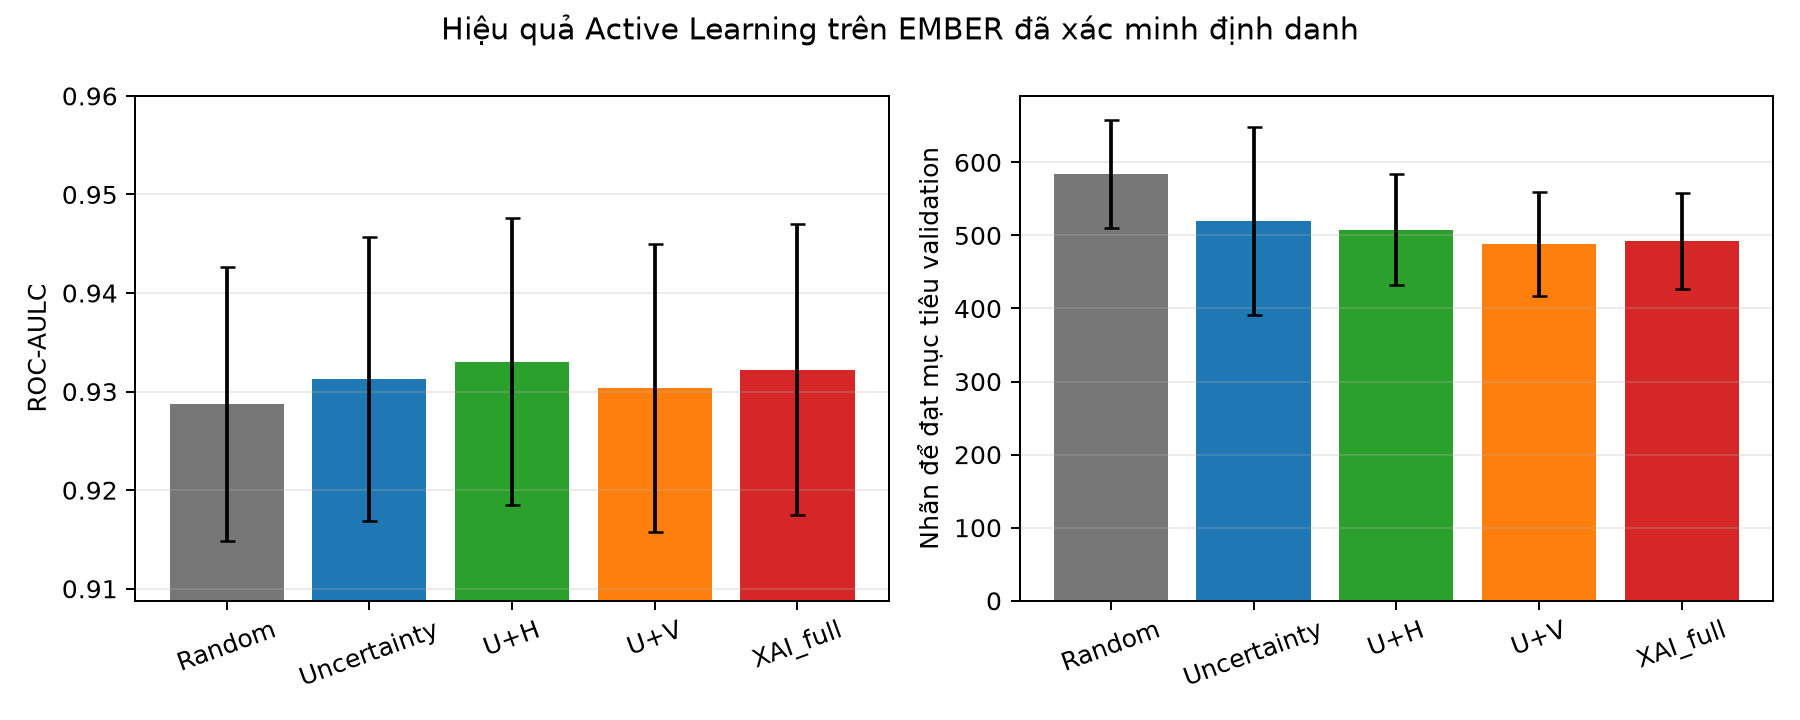
\includegraphics[width=\linewidth]{assets/al_metrics.png}

\column{0.34\textwidth}
\small
\begin{bluebox}{Hiệu quả sử dụng nhãn}
\begin{itemize}\smallbullet
  \item XAI-full đạt mục tiêu với \keynum{492 nhãn}.
  \item Random: 584 $\Rightarrow$ tiết kiệm \good{92 nhãn (15,8\%)}.
  \item Uncertainty: 520 $\Rightarrow$ tiết kiệm \good{28 nhãn (5,4\%)}.
\end{itemize}
\end{bluebox}

\vspace{0.15cm}
\begin{bluebox}{Chất lượng đường học}
U+H -- Random: $\Delta$ROC-AULC \keynum{+0,00425}; $\Delta$AP-AULC \keynum{+0,01498}; thắng 5/5 folds. Overhead query của XAI-full: \warn{5,42\%} train+query.
\end{bluebox}
\end{columns}
\source{al/aulc\_summary.csv; target\_reach\_summary.csv; overhead\_by\_fold.csv; 25 cặp fold--seed.}
\end{frame}

% 10
\begin{frame}[t,shrink=8]{Đóng góp 3 — Fidelity và độ ổn định của SHAP}
\begin{columns}[T,onlytextwidth]
\column{0.64\textwidth}
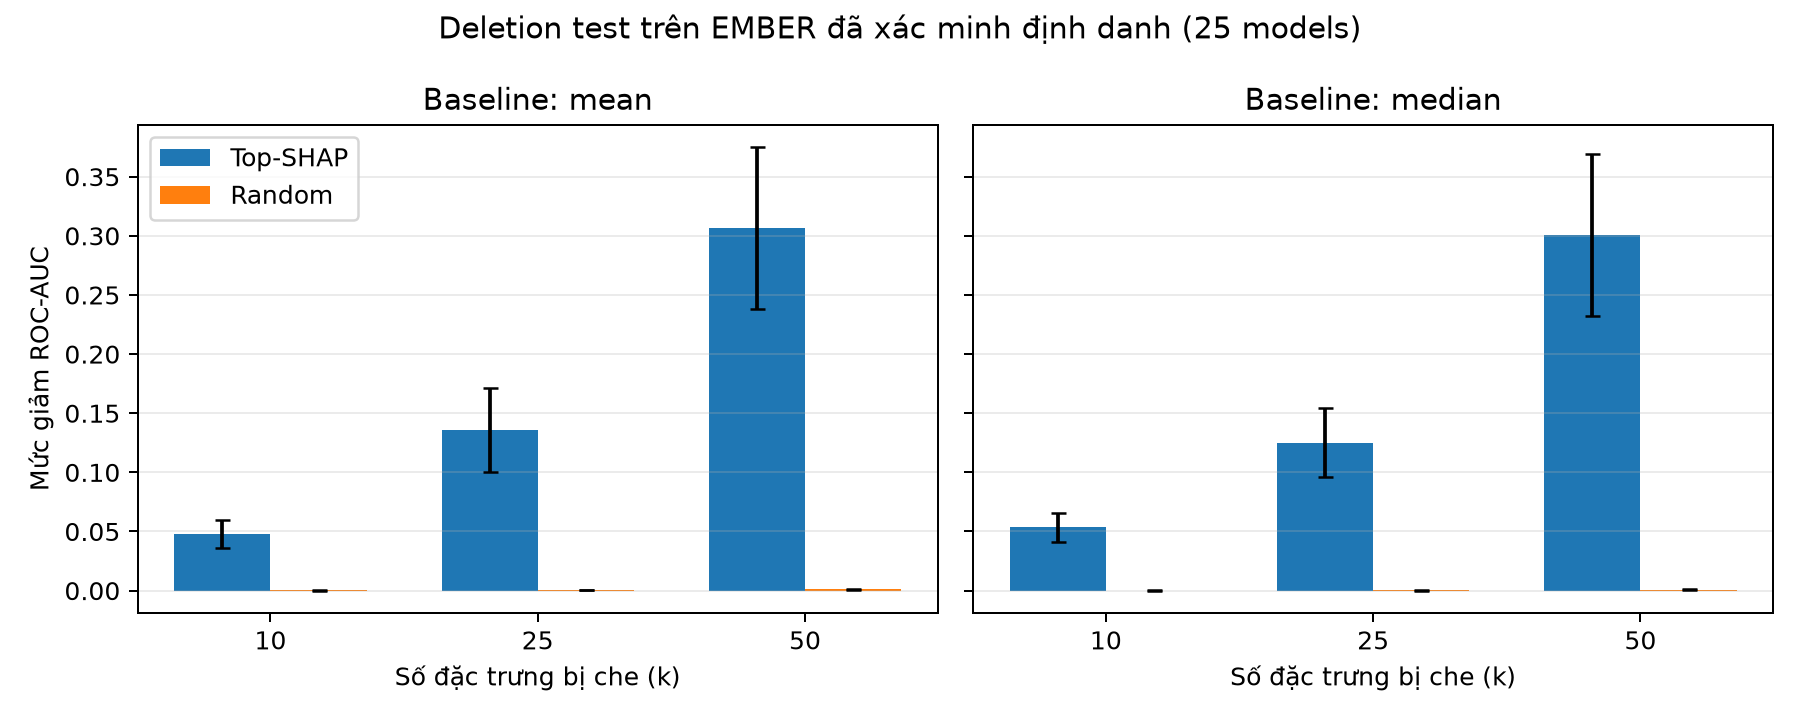
\includegraphics[width=\linewidth]{assets/fidelity_deletion.png}

\column{0.34\textwidth}
\small
\begin{bluebox}{Deletion test — mean baseline}
\begin{itemize}\smallbullet
  \item $k=10$: top-SHAP \keynum{0,0478}; random 0,0002.
  \item $k=25$: top-SHAP \keynum{0,1359}; random 0,0005.
  \item $k=50$: top-SHAP \keynum{0,3067}; random 0,0010.
\end{itemize}
\end{bluebox}

\vspace{0.13cm}
\begin{bluebox}{Consistency}
Spearman thứ hạng: \keynum{0,614} trong fold và \keynum{0,551} giữa các fold. Kết quả cho thấy SHAP bám vào hành vi mô hình trong không gian đặc trưng EMBER.
\end{bluebox}
\end{columns}
\source{fidelity/deletion\_summary.csv; shap\_stability\_summary.csv; 25 models, mean/median masking.}
\end{frame}

% 11
\begin{frame}[t,shrink=8]{Tiếp thu góp ý của Hội đồng Seminar}
\begin{columns}[T,onlytextwidth]
\column{0.58\textwidth}
\scriptsize
\renewcommand{\arraystretch}{1.28}
\begin{tabularx}{\linewidth}{>{\bfseries}p{2.45cm} X}
\toprule
Góp ý Seminar & Nội dung đã bổ sung \\
\midrule
Tách đóng góp từng thành phần & Ablation PID; U/H/V; top-SHAP so với random \\
Kết quả gán nhãn chưa thuyết phục & 5 folds $\times$ 5 seeds; AULC, số nhãn tới mục tiêu, overhead \\
AUC tăng ít có ý nghĩa gì? & Chênh lệch ghép cặp, CI, AP và FPR/TPR \\
Độ đo XAI có phù hợp? & Mean/median masking, ba mức $k$, stability; không gộp OFS \\
Tổng thể hệ thống được gì? & Đối chiếu từng claim với artifact và ablation \\
\bottomrule
\end{tabularx}

\column{0.39\textwidth}
\begin{bluebox}{Bằng chứng đã khóa trong deck}
\small
\good{AL: đã xác nhận.}\\[1mm]
\good{Fidelity: đã xác nhận.}\\[1mm]
\good{PID: đã đo trên 199 mẫu ghép cặp.}
\end{bluebox}

\vspace{0.16cm}
\begin{bluebox}{Giới hạn phát biểu}
\small
\begin{itemize}\smallbullet
  \item PID là bằng chứng thăm dò trên MalBehavD-V1, không đại diện riêng cho ransomware.
  \item Không tuyên bố thành phần D làm giảm FPR.
  \item Không gộp Fidelity thành OFS khi trọng số chưa được kiểm định.
\end{itemize}
\end{bluebox}
\end{columns}

\end{frame}

% 15
\begin{frame}[t]{Kết luận: Ba đóng góp và giá trị thực nghiệm}
\begin{columns}[T,onlytextwidth]
\column{0.32\textwidth}
\begin{bluebox}{1. PID Fusion}
\small
Kết hợp tĩnh--động nâng AUC từ 0,9254/0,9345 lên khoảng 0,958--0,959. Trên cohort này, $P$ đủ mạnh; lợi ích riêng của $I/D$ chưa rõ.
\end{bluebox}

\column{0.32\textwidth}
\begin{bluebox}{2. XAI-Guided AL}
\small
XAI-full đạt mục tiêu với 492 nhãn: giảm 92 nhãn so với Random và 28 nhãn so với Uncertainty; U+H cải thiện AULC ở 5/5 folds.
\end{bluebox}

\column{0.32\textwidth}
\begin{bluebox}{3. Fidelity}
\small
Che top-50 SHAP làm AUC giảm 0,3067, trong khi random chỉ 0,0010; Spearman đạt 0,614 trong fold và 0,551 giữa fold.
\end{bluebox}
\end{columns}

\vspace{0.28cm}
\begin{bluebox}{Thông điệp chính}
Giá trị của luận văn nằm ở ba phép kiểm chứng bổ sung cho nhau: dung hợp hai nguồn tín hiệu, giảm chi phí nhãn và kiểm tra lời giải thích bằng hành vi mô hình. Kết quả được báo theo artifact, ablation và khoảng tin cậy thay vì dựa vào một con số Accuracy.
\end{bluebox}

\vfill
\centering{\Large\bfseries\color{uetblue}Xin trân trọng cảm ơn Hội đồng!}
\end{frame}

\end{document}
